\chapter{}
Monique's final week in the hip spica went well. After three weeks of coping with her
extensive immobilization, we'd gotten quite good at dealing with the situation we'd been
``forced'' into.

Of course, we had the weekends free, but her cast defined our lives five days of the week.
We started to realize how people forced into similar situations dealt with it. You quickly learn
what is possible, what isn't, and what concessions you have to make. Helping Monique with her
rest room needs had been awkward at first, but by the time we cut her out of the last hip spica,
it was no longer anything either of us really thought about.

School had even become routine. Getting her in and out of the vehicle had become quite
easy, and moving her to her classes in the wheelchair had gotten enjoyable. Of course, our
confidence that the ruse was completely accepted as truth had put us at ease, and allowed us to
go through the days enjoying the people around us; the ones we'd had contact with throughout the
ordeal hardly mentioned it, except the occasional question about how much longer she'd be
wearing the cast, or when the next doctor appointment was. Of course, the best part was seeing
people that we hadn't seen before. Their responses ranged from stares to the flurry of questions
we'd answered dozens of times already.

\begin{thought}
As they headed home on Friday, Monique was a little bit sad. The three weeks in school in
the big cast had been a lot of fun. While there had been many challenges, the experience had
been very enjoyable. She'd known all along that it had to end, but she wasn't quite ready for it
to end just yet. The whole experience of playing out the charade behind the cast had been a
thrill. The risk of being found out made it even more exciting. Pretending to be badly injured
and in a huge, unrealistic cast was something she definitely wanted more of.
\end{thought}

When we'd cut the cast off, her movement was shockingly slow and pained. She tried to play
it off and minimize it, but she was very noticeably stiffer and weaker than last week. I was
glad that we were abandoning the hip spica part of the charade. I was hoping we'd do another hip
spica again, but not for such a long time, and we'd make sure she had plenty of time to recover
from this one before I'd even dream of doing one again.

I had to help her to the tub for a soak, as she was just a bit too wobbly for me to trust
her climbing the stairs alone.

\begin{thought}
Monique sat in the tub for at least an hour, letting the warm water loosen up her aching
joints and muscles. When the water started to cool, she drained some off and refilled it with
more hot water. When she was done, her joints no longer ached as badly, but her muscles were
still achy, weak and twitchy. Maybe three weeks of immobility was a bit much. She certainly had
no desire to be back in a hip spica any time in the near future, though she knew that feeling
would pass as she recovered from this adventure.
\end{thought}

We spent the rest of the evening just relaxing. I wasn't anxious to see Monique hit any
exercise equipment that evening, and thankfully, neither was she. When it was time for bed, she
was able to make it upstairs on her own. The effects were still visible, but she was certainly
better than she'd been earlier.

Saturday morning, Monique started slowly exercising. Thankfully, she was quickly regaining
flexibility. Though she had to have lost some muscle tone, her legs still looked great. While
looking at her legs, I began thinking about decisions we'd need to make soon, and over lunch, I
brought them up:

``Monique, we need to decide what the next stage of your `treatment' is going to be.''

``I know,'' she replied. ``What were you thinking?''

``Well,'' I started. ``You know that I find you unbelievably sexy in casts.''

She smiled.

``But, I love you. And those feelings are more important than any hardware you may or may
not wear. These past three weeks have been a LOT of fun. I've enjoyed them quite a bit. But, it
has hurt me to see you in pain when we cut you out after a week of immobility.''

``The pain isn't a big deal.'' She said. ``I've enjoyed the time in the hip spica more than I
expected to. I know we have to end that part of this game, but the game can't be over, either.
It wouldn't fit with the story I've been telling.''

``I know that. So, what does fit? What are our options?''

``Well, from the story I've told, the hip and pelvis can be healed enough to be free, and I
think we both agree that we need to go that route.''

``Yes,'' I agreed.

``Mind you, I want more hip spicas, but not right now,'' she added with a smile. ``The right
leg and ankle were mostly healed at the last checkup, so I could go forward with a long leg
cast, a short leg cast, one of the new camwalkers, or nothing at all on the right leg. The left
leg was the slowest to heal, with a tib/fib fracture. We have the same options for the left leg,
except for nothing. We have to do at least a camwalker or short leg cast on that one.''

``Do you have a preference?'' I asked.

``Why not a long leg cast on the left, and a short leg cast on the right?'' Monique asked.

``I was thinking more like a camwalker on the left leg, and the right one free. You've been
really immobile for a while. I'd like something that frees you up every night. I don't want this
giving you any more problems. I want all of our playing with plaster (and fiberglass) to be all
about fun and enjoyment.''

\begin{thought}
Monique knew he was right, but she still wanted to be a spectacle. She enjoyed the
attention, and she didn't think that a single cam would get the attention she wanted. This
experience of being the ``poor injured girl'' had been a lot of fun. She knew that they couldn't
do it again without being obvious that something deceptive was going on. She wasn't ready for it
to end, even though she knew it had to be ratcheted down, and further down than what she wanted.
\end{thought}

``How about a compromise?'' she suggested.

``What did you have in mind?''

``A cam on the right, a plaster short leg walking cast on the left.''

``Why not two camwalkers? Then you can be totally free whenever you're not in public.'' I
couldn't believe we were actually negotiating casts.

``I really want to keep some hardware.'' She said. ``And deep down, you want me too, also.
Admit it.'' She flashed that smile of hers with the last part.

``Okay, but the short leg cast will be fiberglass.'' I relented. ``It's lighter, easier on
you, and you can still walk on it immediately if we change it every weekend.''

She agreed.

Sunday afternoon, she suggested that we go ahead and get her ready for Monday, then go out
for dinner. I agreed. Soon, she had changed into shorts, and was sitting on the casting table in
front of me. I unrolled stockinette up her leg past her knee, and clipped it off past her toes.
I wrapped two rolls of four inch padding, making sure to pad extra around her ankle. This was
more important on this cast than any other one I'd ever done, since she would not only be
walking on this cast, but would be walking on it for a week.

\begin{thought}
The familiar fruity smell filled Monique's nose as Quinn wrapped the red fiberglass on her
leg. She knew that her new cast and camwalker would draw attention, if only because they were
such a change. She was going to miss the big cast, but she knew there would be more of them, and
knew she'd be able to talk Quinn into going into public with them.
\end{thought}

Once the cast was done, I retrieved the camwalker, and undid the straps. I wrapped the foam
padding around her right leg, and then cinched the straps. I retrieved Monique's crutches, and
she gimped around as she waited for the fiberglass to fully cure. After about an hour, I
strapped a cast shoe over the cast, and she tried walking without the crutches, which was more
than a bit awkward for her. I gave her the crutches back, and she worked a bit, finding a way to
walk on both legs, using the crutches.

We decided to head out for dinner, and as we walked outside, a chilly breeze hit us. Fall
was definitely coming.

``Whoa,'' Monique said. ``It's a little cool for shorts and a t-shirt. Hang on while I go
change.''

``Will you be okay on the stairs?:''

``Yeah, I'll be fine.'' She said over her shoulder as she headed inside.

\begin{thought}
After slowly, but successfully negotiating the steps, Monique quickly slipped out of her
shorts and t-shirt. She selected a striped sweater, and put it on, then started going through
her jeans for a pair with wider cuffs. She found the pair she wanted, then sat down, She
released the straps, and took off the camwalker and the cast shoe. She worked the jeans over the
cast, and stood up and fastened them. She wanted the cast and the camwalker to be visible, so
she rolled both legs up to the knees, and then strapped the cast shoe and camwalker back on. She
then rejoined Quinn, and they headed off to dinner.
\end{thought}

At dinner, Monique was approached by a young woman she shared a class with. I watched as
Monique crafted the next chapter of the story with her answers to the questions she faced.

``Wow! It must be great to be out of the body cast!''

``Yes,'' Monique answered.'' It feels good to be able to move around so much more. I'm still
stiff and weak, but I'm working on building my strength back up where I can. And sleeping is so
much more comfortable!''

``You're not missing that wheelchair much either, I bet.''

``Well, I'm not completely done with it. The doctor says to take it easy. I can't do
anything terribly strenuous with my legs at all, and he says that I can only do crutches as long
as there's no pain. I have to go back to the chair if I start hurting.'' I noticed that she was
leaving herself an opening to keep using the wheelchair whenever she wanted.

How long do you have to wear those? She asked, pointing to Monique's legs.

``Well, the right leg is almost completely healed,'' Monique started. ``I can even take this
boot thing off when I sleep.'' The left leg still has some time to go. I go back for more x-rays
in three weeks.''

They talked a few minutes about their common class, and then the girl left. We finished our
dinner and headed home.

At home, we discussed the plans for the next day. We'd have her in the wheelchair, with the
story being that she wanted to be careful, and didn't want to be caught out without the
wheelchair if she started having pain. As we talked, she sat on the couch with her feet up. I
liked the pose, and so I sketched her there as we planned the next day.

All week long, the news about Monique had bothered Diane. She'd been angry when Monique had
told her over the phone that she wasn't going to move back in. She was also shocked. Monique had
always been responsible, and to do something like that, with no warning, and over the phone was
completely unlike anything she'd ever expect from her. The news that she'd been so badly hurt
was a shock, too. Why hadn't Monique told her? She'd spent the week keeping an eye out at school
for her, hoping to bump into her, but she hadn't seen her. She'd tried Monique's cell phone, but
had gotten a pre-recorded message about the number not being in service. Monique had stopped
buying minutes when money got tight, and apparently still hadn't been able to reactivate it. She
called Shawna, the girl who had seen Monique and told her about her being injured.

``Hello?''

``Hi Shawna, it's Diane.''

‘'Hi Diane, what's up?''

``I'm just worried about Monique. It's just weird that she didn't tell me she was hurt.''

``I don't know why she wouldn't.''

``Me either. Where did you see her at? At what time? I want to talk to her- see how she's
doing.''

``I saw her out by the statue, eating lunch with her boyfriend. I think it was on a Tuesday,
but I'm not sure.''

``Is her boyfriend anyone I would know?''

``I don't think so. I've never seen him before. He's a little older than we are.''

``What's his name?''

``I think she said it was Quinn.''

Diane paused for a second, a bit startled.

``Diane, are you there?'' Shawna asked.

``Yeah, yeah. Sorry. You said it was Quinn. Are you sure?''

``Yeah, it stuck out, partly because it was so odd, and partly because he's kinda cute. Why,
do you know him?''

``I think I introduced them.''
\newpage
\begin{center}
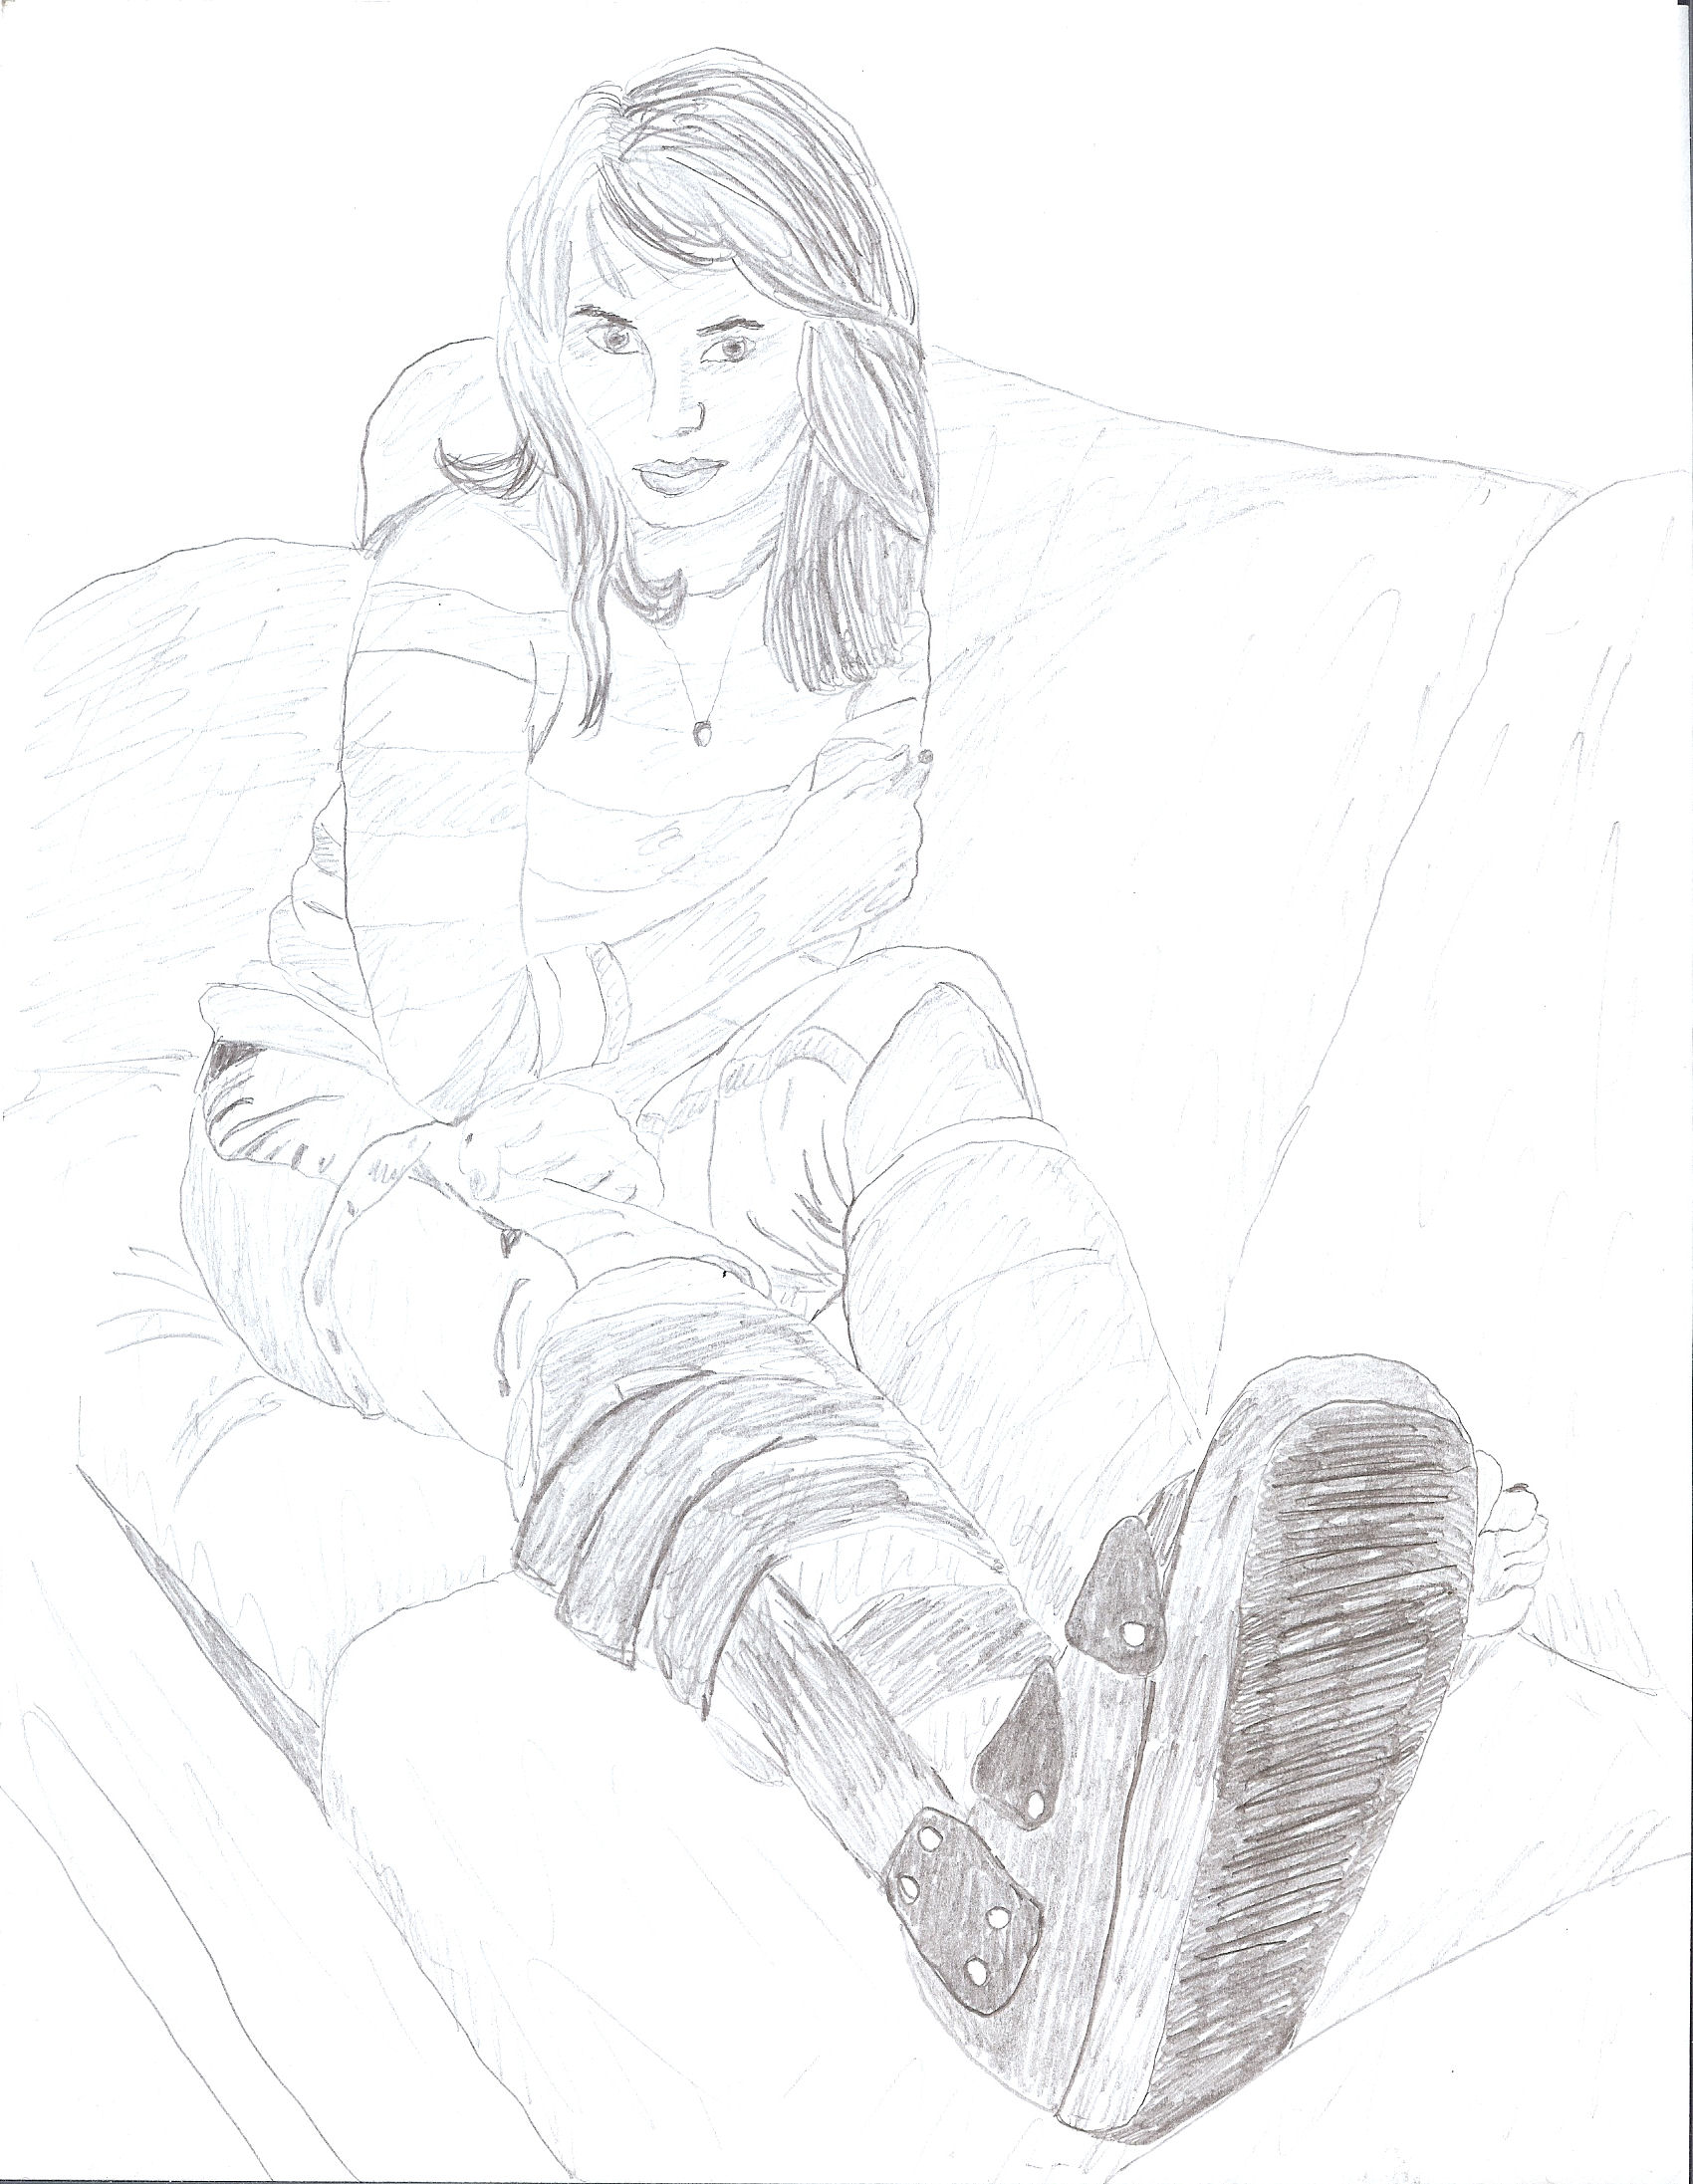
\includegraphics[height=0.8\textheight]{images/kicks49.jpg}
\end{center}
